%%%%%%%%%%%%%%%%%%%%%% DOKUMENT_HEADER %%%%%%%%%%%%%%%%%%%%%%%%%%%%%%%%%
\documentclass[a4paper, 10pt]{article}

%-------------------------- Packete ------------------------------------
\usepackage[english]{babel}
\usepackage{graphicx}
%\usepackage{a4wide}        % seiten mehr ausf�llen
\usepackage{amsfonts}
\usepackage{amsmath}
\usepackage{amssymb}
\usepackage{fancyhdr}
\usepackage{color}
\usepackage[colorlinks=false,linkbordercolor=0 0 0]{hyperref}
\usepackage{tikz}
\usepackage{algorithmic}
\usepackage{algorithm}
\usepackage{fp}
%\usepackage[pdftex,pdfstartview=FitB,colorlinks=true,citecolor=black,
%urlcolor=black,linkcolor=blue,pdfpagemode=None]{hyperref}

\tikzstyle{normalnode}=[draw,%
                          rectangle,%
                          shade,%
                          minimum size  = 1.0cm,%
                          node distance = 1.3cm]
 \tikzstyle{normalnode2}=[draw,%
                          rectangle,%
                          shade,%
                          minimum size  = 1.0cm,%
                          node distance = 1.0cm]
  \tikzstyle{start}=[draw,fill=green!70,rectangle, minimum size=1.0cm,node distance=1.3cm]                        
  \tikzstyle{goal}=[draw,fill=red!70,rectangle, minimum size=1.0cm,node distance=1.3cm]
  \tikzstyle{goal2}=[draw,fill=red!70,rectangle, minimum size=1.0cm,node distance=1.0cm]
  \tikzstyle{agent}=[draw,fill=blue!70,circle,minimum size=0.6cm]
  \tikzstyle{dummy}=[circle]


%------------------------- Einstellungen -------------------------------
\setlength\parskip{\medskipamount}
\setlength\parindent{0pt}

%================== Kopfzeilenlayout ====================
\pagestyle{fancy}
%\renewcommand{\chaptermark}[1]{\markboth{\chaptername\ \thechapter.\ #1}{}}
%\renewcommand{\sectionmark}[1]{\markright{\thesection\ #1}{}}
\fancyhf{}
\fancyhead[LE,RO]{\thepage}
\fancyhead[RE]{\sffamily \rightmark}
\fancyhead[LO]{\sffamily \leftmark}
\fancyfoot{\sffamily}
\pagestyle{fancy}

%_-------------------------Definitionen---------------------------------
\newcommand{\FO}{\textrm{FO}}      % romanstyle FO
\newcommand{\cL}{\mathcal{L}}      % kalligraphisches L
\newcommand{\cC}{\mathcal{C}}      % kalligraphisches C
\newcommand{\N}{\mathbb{N}}        % nat�rliche Zahlen N
\newcommand{\gdw}{\Leftrightarrow} % genau dann wenn \gdw
\newcommand{\folgt}{\Rightarrow}   % \folgt f�r daraus folgt Pfeil
% \eodef \eobew
% Liefert einen rechtsbuendigen Kasten zur Kennzeichnung des Endes einer 
% Definition (leer) und eines Beweises (ausgefuellt).
\newcommand{\eobew}{\par\begin{flushright}$\square$\end{flushright}}
\newcommand{\eodef}{\begin{flushright}$\blacksquare$\end{flushright}}
\newcommand{\argmax}[1]{\underset{#1}{\operatorname{argmax}}\;}
\newcommand{\argmin}[1]{\underset{#1}{\operatorname{argmax}}\;} 
\DeclareMathOperator*{\argmin}{argmin}
\DeclareMathOperator*{\argmax}{argmax}

%%%%%%%%%%%%%%%%%%%%%%%%%%%%%%% DOKUMENT %%%%%%%%%%%%%%%%%%%%%%%%%%%%%%%
\begin{document}

%%%%%%%%%%%%%%%%%%%%%%%%%%%%%% TITELSEITE %%%%%%%%%%%%%%%%%%%%%%%%%%%%%%
 \begin{titlepage}
     \begin{center}
       \large
       \textsc{Rheinisch-Westf\"alische Technische Hochschule Aachen}\\
       Knowledge-Based Systems Group \\
       Prof. G. Lakemeyer, Ph.D. \\ 
       \vspace{3 cm}
       \huge Seminar Foundations of AI\\
       \large summer term 2009 \\
       \vspace{1 cm}
       \huge
       Multi-Agent Reinforcement Learning\\
       \vspace{4 cm}
       \Large Christian Kalla\\
       \vspace{3 cm}
       last build: \today \\
     \end{center}
 \end{titlepage}

%\title{Multi-agent Reinforcement Learning}
%\date{\today}
%\author{Christian Kalla}
%\maketitle

%\clearpage
%% %%%%%%%%%%%%%%%%%%%%%%% INHALTSVERZEICHNIS %%%%%%%%%%%%%%%%%%%%%%%%%%
\tableofcontents
\clearpage

%% %%%%%%%%%%%%%%%%%%%%%%%%%%%%%%%%%%%%%%%%%%%%%%%%%%%%%%%%%%%%%%%%%%%%%
\section{Introduction}
\label{sec:intro}
Reinforcement Learning can be regarded as one of the most natural ways of learning by interacting with the environment.\\
In contrast to other methods of machine learning, an agent only learns by receiving feedback from its environment and trying out which actions yield the highest return in a certain situation. It does not seem astonishing at all that one of the roots of this method of learning can be found in psychology. An illustrative example is comparing this method to the way infants learn when making their first steps in an unknown environment. For example crying will often lead to the result that the parents get something to drink or to eat for the child, which can be regarded as a reward. So crying would be learned as a good action when trying to reach the goal of getting food.  Another analogy is the situation when learning to drive (also referred to in \cite{Markelic04reinforcementlearning}). Neglecting the driving instructor who could turn this example into one for supervised learning, driving can also be learned by paying attention to the reactions of the environment (e.g. the car and other road users). One goal could be to get no bad reaction of the other drivers, so honking could be a bad signal from the environment and remind you to drive faster for example. More of those analogies can be found in \cite{Sutton98}.\\
One important fact is that the aim of an agent is always to maximize the sum of rewards on the way to its goal and not to focus on single rewards. This stresses the need of a so called value function that tells the agent how good certain states are with respect to the expected sum of rewards.\\
The first section of this paper will deal with methods and algorithms to compute this value function and point out the occuring difficulties and will conclude with an overview of some interesting applications. In this context Markov Decision Processes (see \cite{Barto90learningand},\cite{Howard60}) play an important role which assume a stationary environment that does not contain other adaptive agents. The arising problem from this is that cooperation of agents that would be important for many multiplayer games cannot be considered as it is not supported by the mathematical framework.\\
This problem is regarded in the second section of this paper mainly considering the work of \cite{Littman94}. Here Markov Games which explicitely support multi-agent environments are used to adapt the Q-Learning algorithm presented in the first section to develop an agent for a simple version of soccer. The corresponding algorithm will be presented and the results against other agents will be shown and discussed.

%% %%%%%%%%%%%%%%%%%%%%%%%%%%%%%%%%%%%%%%%%%%%%%%%%%%%%%%

\section{Foundations of Reinforcement Learning}
\subsection{The main idea behind reinforcement learning}
The general idea of reinforcement learning is visualized in Figure \ref{agentWorldModel}. An agent starts at time $t$ in a given state $s_{t}$ and chooses an action $a_{t}$ ($a_{t} \in \mathcal{A}(s_{t})$). This action takes him to a new state $s_{t+1}$ and gives a reward $r_{t+1}$ as feedback. The new state and the reward depend on the dynamics of the environment and may be deterministic or stoachastic. This means that the rewards and successor states are either clearly defined (e.g. in games like chess) or occur with a certain probability (this could be the case in real-time environments). In many scenarios the reward is often not given directly, but when reaching the goal. This often leads to the problem that an agent does not know how good his actions were before having reached the goal state for the first time.
\begin{figure}
\centering
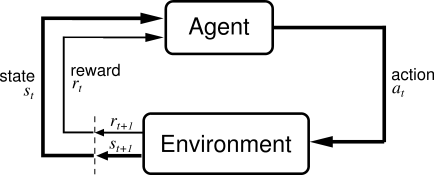
\includegraphics[scale=0.5]{pics/worldModel.png}
\caption{The model of the agent and its environment for reinforcement learning (taken from \cite{Sutton98})}
\label{agentWorldModel}
\end{figure}
\subsection{Separation from other Machine Learning Techniques}
This section gives a comparison of reinforcement learning and other machine learning techniques.
Machine learning in general distinguishes between three learning approaches: Supervised learning, unsupervised learning and reinforcement learning. The main task of all those approaches is to use the knowledge gained from previous experience to solve new tasks using this knowledge.\\
In supervised learning the agent is given a set of examples containing input and the correct output. After that the agent adapts the parameters of its model (e.g. the parameters of a probability distribution) in such a way that the seen data is represented best. This is often done by the maximum likelihood method. One example for this kind of learning could be the recognition of handwritten letters or digits, where the agents gets some example images with the correct letter or digit. After that the model is used to classify some unknown input text.\\
In unsupervised learning the agent is just given the data itself, but not the correct class, so there is no "teacher" as in supervised learning. In order to learn from the data and derive a model, clustering methods and the EM algorithm play an important role.\\
Reinforcement learning differs from both previous approaches, because the agent has to discover its environemnt on its own, without having a supervisor that tells him the correct actions. The only feedback if the chosen action was good or bad can be extracted from the reward or punishment the action sequence brings.\\
But which advantages does this approach have?  In \cite{Sutton98} an example of a Tic-Tac-Toe playing agent is given. Everybody knows that this game always ends up with a draw when both players make the best moves, but it could also be the case that the opponent agent shows weaknesses in certain positions, although it might play well otherwise. A standard approach to those kinds of zero sum games is applying the Minimax algorithm with a simple heuristic that guarantees to gain the best result assuming that the opponent always chooses the best move. One disadvantage here is that always optimal play of the opponent is assumed, although this might be wrong. Applying reinforcement learning algorithms to this kind of game would result in an agent that discovers the weaknesses of its opponent and exploits, whereas a minimax approach would just be able to reach a draw for example.
\subsection{Important Problems}
\paragraph{Problem of Exploration and Exploitation}
A difficult task for an agent in an environment is to find the right balance between using the information gained by already visited states (e.g. the values of states in the reinforcement learning case) and trying to explore the environment by taking actions leading to unknown states. One problem that can occur during reinforcement learning is that once the agent has found a way to the goal, it will always use the same way again, without knowing if there is another (probably better) one. We all know this problem when driving to work for example being annoyed about traffic jams, for example. Of course one way found by our initial policy (e.g. the motorway) definitely leads to the goal, but having driven the same way for many times, we try out something new the next day and "explore" the state space in some way. Of course this may also lead to worse results than before, but there also might be faster ways (analogous to better policies) leading to the goal. $\epsilon$-greedy policies are an example for policies that in general choose the action leading to the state with the highest value, but sometimes (with probability $\epsilon$) take random actions.
\paragraph{The prediction and the control problem}
To reach our main goal in reinforcement learning, namely to maximize the long-term reward and reach a goal state (at least in a continuous environment), it is necessary to define values for every state that determine how good a state is in terms of maximizing the future rewards. The task to find optimal values predicting the expected reward is referred to as "Prediction problem" in literature. A related problem making use of the solution for the prediction problem is the control problem. A solution to this problem is a plan (an optimal policy) that tells us in every situation which action to take in order to receive the highest reward in a long-term view. So a solution for the prediction problem would give us directly a solution for the control problem.
\paragraph{Partial observability problem}
Real world environments are often not fully observable, that means that the agent does not exactly know in which state it will end up after performing an action. This could occur if the values of the sensors cannot clearly indicate if the agent is in state A or state B, because the measurements are characteristic for both states. In the case of partial observability "standard" reinforcement learning algorithms are not applicable, but there are other solution methods based on POMDPs (partial observable Markov Decision Processes) (see \cite{pomdp}).
\paragraph{Curse of Dimensionality}
In many environments the state and the action space are to huge to be explored completely. Due to this facts there have to be methods to reduce the dimension of those spaces without losing important information. This could be done by means of state-space abstraction.
\paragraph{Credit Structuring Problem}
As the agent learns by being rewarded or punished, it is also an important task to structure the rewards in such a way that the agent learns fastest. Taking the game of chess as an example, it would make no sense to give a reward for winning material in general, because this could tempt our agent into winning material instead of checkmating the opponent which has to be seen as the main goal. One disadvantage of delaying the reward to the goal state is that it may take a very long time until the agent reaches this state, because there is no indicator in form of rewards that lead the agent to the final state. This is why learning could take very long, because the state sequence to the goal state in games like chess is very long, also because of the fact that the agent just makes random moves at the beginning, because it has not developed a policy yet. This is why assigning rewards to states is not an easy task at all.
\paragraph{Non-stationary environments}
This problem addresses the fact that the environment sometimes changes during learning. So a value function learned for a high number of episodes could be wrong, because the dynamics of the envirionment have already changed in the meantime. If the change of the environment is too fast, learning is no longer possible. Nevertheless, not only reinforcement learning methods, but learning in general is affected by this problem.
\subsection{Value Function and Policies}
As mentioned before, the main goal of an agent is to find an optimal policy $\pi^{*}$, i.e. a roadmap that enables the agent to choose the right action in each state in order to reach its goal as fast as possible. Or more formally:
\newtheorem {definition} {Definition}
\begin{definition}[Policy]
Let $S$ be a set of states and $A$ be a set of actions an agent can choose in its environment.\\
A mapping $\pi:S \rightarrow A \ for\ all\ s \in S$ is called a policy .
\end{definition}
\begin{definition}[Optimal Policy]
A policy $\pi^{*}$ that maximizes the quantity
\begin{equation}
R=r_{0}+r_{1}+...+r_{n}
\end{equation}
for Markov decesion processes (MDPs) with a terminal state or the quantity
\begin{equation}
R=\sum_{t}{\gamma^{t}r_{t}}
\end{equation}
for MDPs without a terminal state ($0 \leq \gamma \leq 1$ denotes the discounting factor) is called an optimal policy.
\end{definition}
In order to find optimal policies, a value function that defines the value of a state itself (V-function) or the value for choosing an action in a given state (Q-function) is needed. As the value of a state always depends on the expected future reward, it depends also on the future actions taken by the agent. That is why value functions always have to be considered with respect to a certain policy (denoted by the index $\pi$). More formally:
\begin{definition}[State-value function]
The function
\begin{equation}
V^{\pi}(s)=E_{\pi}\left\{R_{t}|s_{t}=s \right\}=E_{\pi}\left\{ \left. \sum_{k=0}^{\infty}{\gamma^{k}r_{t+k+1}}\right|s_{t}=s  \right\}
\end{equation}
is called the state-value function for policy $\pi$. $E_{\pi}{}$ denotes the expected value given the fact that the agent follows the policy $\pi$ with an arbitrary time step $t$.
\end{definition}
\begin{definition}[Optimal state-value function]
The function
\begin{equation}
V^{*}(s)=\max_{\pi}{V^{\pi}(s)} \forall s \in \mathcal{S}
\end{equation}
is called optimal state-value function.
\end{definition}
The action-value function $Q^{\pi}(s,a)$ that assigns values to a state-action pair is defined similarly:
\begin{definition}[Action-value function]
The function
\begin{equation}
Q^{\pi}(s,a)=E_{\pi}\left\{R_{t}|s_{t}=s, a_{t}=a \right\}=E_{\pi}\left\{ \left. \sum_{k=0}^{\infty}{\gamma^{k}r_{t+k+1}}\right|s_{t}=s, a_{t}=a  \right\}
\end{equation}
is called the action-value function for policy $\pi$. 
\end{definition}
\begin{definition}[Optimal action-value function]
The function
\begin{equation}
Q^{*}(s,a)=\max_{\pi}{Q^{\pi}(s,a)} \forall s \in \mathcal{S}\ and \ a \in \mathcal{A}(s)
\end{equation}
is called optimal action-value funciton.
\end{definition}
As the goal of reinforcement learning is to find an optimal policy from the initial state to the goal, there have to be methods to compute an optimal policy efficiently. A naive way to do so would be trying out all possible policies which means taking every possible action in every state and receiving the rewards from the environment. Of course the complexity of this approach would be too high, because the set of states and the set of actions are very large in general, so exploring the whole search space is inefficient. There are many methods to approximate optimal value functions and therefore also give an approximation for an optimal policy. The first two methods that will be presented use dynamic programming and perform policy or value iteration. This means to start with an arbitrary policy for example, determine the resulting value function for this policy and use this value function to get an improved policy. After this the same procedure is iterated several times until the optimal policy is found (or at least a good approximation). A significant disadvantage of those dynamic programming methods is that they require a complete model of the environment and so they are not applicable if the environment is unknown to the agent.\\
In contrast Monte-Carlo methods do not require this model. Here the value function is learned by averaging the rewards of many episodes. Because the transition probabilities of the environment are not known (in contrast to DP methods), they have to be determined by many iterations.\\
Another important kind of reinforcement learning algorithms do not require this environment model and use Temporal Difference learning. This means that they compute the difference between the two values of a value function at different time points (e.g. $Q(s,a)-Q(s',a')$). The presented algorithms Q-learning and SARSA are two examples for this kind of learning method.
\subsubsection{$\epsilon$-greedy Policy}
In order to derive a policy from the value function, it makes sense to choose the action that maximizes the value of the successor state. But in order to guarantee an optimal exploration of the state space, an $\epsilon$-greedy policy chooses a random action with probability $\epsilon$ instead of trying to choose the "best" action in terms of the highest value of the successor states. Those kind of policies are often used in reinforcement learning algorithms.
\subsection{The Markov Property and Markov Decision Processes}
The goal of reinforcement learning is to maximize an agents reward and to find an optimal policy leading to a goal state. But how do environments behave, if an agent chooses an action in a state at a given time? The first thing we have to consider when answering this question is to imagine different environments and think about their characteristics. At this point we have to distinguish between deterministic and stochastic environments. Playing chess is an example for a deterministic environment. There is a specified choice of actions in each state and each of those actions leads to a clearly defined next state. The environment we live in does not necessarily lead to one defined state when taking an action. Instead an action could lead to several states and each of those successor states can occur with a given probability. For example the state "Driving drunk" with the action "Driving in an erratic manner" could lead to the state "Getting stopped by the police", but also to the state "Arriving safe at home". Another important question is if the probability of the successor states depends on the actions taken before, or if just the current state counts for future decisions. This is exactly what the Markov Property demands. For the chess example this question is easy to answer: The agent has to make his decision based on the current position (i.e. the current state) and the environment also does not care about what happened in the past. For other kinds of environment this conditional independence from earlier states cannot be guaranteed in many cases. One thing that might be confusing in this context is the definition of a state itself. The definition of a state takes information about the agents' sensors as input, so a state can depend from sensations made somewhen earlier. The Markov property can formally be expressed as follows:
\begin{equation}
\begin{align}
&Pr\left\{s_{t+1}=s',r_{t+1}=r|s_{t},a_{t},r_{t},s_{t-1},a_{t-1},...,r_{1},s_{0},a_{0}\right\}\\
=&Pr\left\{s_{t+1}=s',r_{t+1}=r|s_{t},a_{t}\right\}
\end{align}
\end{equation}
Every reinforcement learning task whose states have the Markov Property is called a Markov Decision Process (MDP). If the state and action space are finite we talk about finite MDPs. MDPs are formally defined in \cite{Howard60} and consist of the following components:
\begin{itemize}
\item a set of states $\mathcal{S}$
\item a set of actions $\mathcal{A}$
\item a set of rewards $\mathfrak{R}$
\item a transition function $T:\mathcal{S}\times \mathcal{A}\rightarrow PD(\mathcal{S})$ where $PD(\mathcal{S})$ denotes the set of probability distribution over $\mathcal{S}$
\item a reward function $R:\mathcal{S} \times \mathcal{A} \rightarrow \mathfrak{R}$
\end{itemize}
In stochastic environments the successor state is not only defined by an action, but also by a probability distribution defining the transition probabilities:\\
\begin{equation}
\mathcal{P}_{ss'}^{a}=Pr \left\{s_{t+1}=s'|s_{t}=s,a_{t}=a \right\}
\end{equation}
Accordingly the expected value of the next reward can be defined as
\begin{equation}
\mathcal{R}_{ss'}^{a}=E \left\{r_{t+1}|s_{t}=s,a_{t}=a,s_{t+1}=s' \right\}
\end{equation}
\subsection{How to find optimal Policies?}
This section gives an overview of algorithms to compute optimal policies.
\subsubsection{Dynamic Programming}
The most obvious way of finding an optimal policy is using dynamic programming techniques. One way is to start with an arbitrary policy, derive the value function and improve the policy thereafter (policy iteration). Another way is to start with an initial value for all states and adapt this value function iteratively (value iteration).
%\paragraph{Value iteration}
\paragraph{Policy Iteration}
An illustration of the principle of policy iteration can be found in the following figure taken from \cite{Sutton98}.
\begin{figure}
\label{policyIteration}
\fbox{
\begin{equation*}
\pi_{0}\stackrel{evaluation}{\longrightarrow}V^{\pi_{0}} \stackrel{improvement}{\longrightarrow}{\pi_{1}} \stackrel{evaluation}{\longrightarrow}{V^{\pi_{1}}}... \stackrel{improvement}{\longrightarrow} \pi_{*} \stackrel{evaluation}{\longrightarrow}{V^{\pi_{*}}}
\end{equation}
}
\caption{The principle of policy iteration}
\end{figure}
The algorithm in pseudocode is given in \ref{policyIterationAlgorithm}.
\begin{algorithm}[tb]
\caption{Policy Iteration}
\label{policyIterationAlgorithm}
\begin{enumerate}
\item \textbf{Initialization}
\begin{algorithmic}
\STATE $V(s) \in \mathfrak{R}$ and $\pi(s) \in \mathcal{A}$ arbitrarily for all $s \in \mathcal{S}$
\end{algorithmic}
\item \textbf{Policy Evaluation}
\begin{algorithmic}
\REPEAT
\STATE $\delta \gets 0$
\FOR {$s \in \mathcal{S}$}
\STATE $v \gets V(s)$
\STATE $V(s) \gets \sum_{s'}{\mathcal{P}_{ss'}^{\pi(s)}(\mathcal{R}_{ss'}^{\pi(s)}+\gamma V(s'))}$
\STATE $\delta \gets \max(\delta,|v-V(s)|)$
\ENDFOR
\UNTIL{$\delta < \theta$ (a small threshold to be reached)}
\end{algorithmic}
\item \textbf{Policy Improvement}
\begin{algorithmic}
\STATE $policy-stable \gets true$
\FOR {$s \in \mathcal{S}$}
\STATE $b \gets \pi(s)$
\STATE $\pi(s) \gets \arg\max_{a}{ \sum_{s'}{\mathcal{P}_{ss'}^{a}(\mathcal{R}_{ss'}^{a}+\gamma V(s'))}}$
\IF{$b \neq \pi(s)$}
\STATE $policy-stable \gets false$
\ENDIF
\ENDFOR
\IF{$policy-stable$}
\STATE STOP
\ELSE GOTO 2.
\ENDIF
\end{algorithmic}
\end{enumerate}
\end{algorithm}
The example shown in the figures \ref{firstPolicyFigure}-\ref{lastPolicyFigure} underlines how the presented algorithm works. The task of the agent is to get from its starting state (the green square) to the goal (the red square) by moving up, down, left and right. The agent only receives a reward if the goal state is reached (+100), otherwise it does not gain anything (0). The initial policy is deterministic and seems to be quite stupid, but according to the algorithm the agent improves this policy quite fast. The discount factor $\gamma$ is set to $0.9$.
\begin{figure}[tb]
\begin{minipage}[t]{0.475 \textwidth}
\begin{center}
  \begin{tikzpicture}
            \node[start] (a)  {0};
            \node[normalnode][right of=a]  (b) {0};
            \node[goal][right of=b]  (c) {};
            \node[normalnode][below of=a]  (d) {0};
            \node[normalnode][right of=d]  (e) {0};
            \node[normalnode][right of=e] (f) {0};
            \draw [->] (a.south) to  node[right] {\tiny 0}  (d.north);
            \draw [->] (d.east) to node[above] {\tiny 0} (e.west);
            \draw [->] (e.north) to node[right] {\tiny 0} (b.south);
            \draw [->] (b.east) to node[above] {\tiny 100} (c.west);
            \draw [->] (f.west) to node[above] {\tiny 0} (e.east);	
  \end{tikzpicture}
\caption{Initial situation of the grid world with rewards for the actions}
\label{firstPolicyFigure}
\end{center}
\end{minipage}
\begin{minipage}[t]{0.475 \textwidth}
\begin{center}
 \begin{tikzpicture}
            \node[start] (a)  {0};
            \node[normalnode][right of=a]  (b) {100};
            \node[goal][right of=b]  (c) {};
            \node[normalnode][below of=a]  (d) {0};
            \node[normalnode][right of=d]  (e) {0};
            \node[normalnode][right of=e] (f) {0};
            \draw [->] (a.south) -- (d.north);
            \draw [->] (d.east) -- (e.west);
            \draw [->] (e.north) -- (b.south);
            \draw [->] (b.east) -- (c.west);
            \draw [->] (f.west) -- (e.east);	
  \end{tikzpicture}
\caption{situation after one value update}
\end{center}
\end{minipage}
\begin{minipage}[t]{0.475 \textwidth}
\begin{center}
  \begin{tikzpicture}
            \node[start] (a)  {72,9};
            \node[normalnode][right of=a]  (b) {100};
            \node[goal][right of=b]  (c) {};
            \node[normalnode][below of=a]  (d) {81};
            \node[normalnode][right of=d]  (e) {90};
            \node[normalnode][right of=e] (f) {81};
            \draw [->] (a.south) -- (d.north);
            \draw [->] (d.east) -- (e.west);
            \draw [->] (e.north) -- (b.south);
            \draw [->] (b.east) -- (c.west);
            \draw [->] (f.west) -- (e.east);	
  \end{tikzpicture}
\caption{situation after all value updates}
\end{center}
\end{minipage}
\begin{minipage}[t]{0.475 \textwidth}
\begin{center}
  \begin{tikzpicture}
            \node[start] (a)  {72,9};
            \node[normalnode][right of=a]  (b) {100};
            \node[goal][right of=b]  (c) {};
            \node[normalnode][below of=a]  (d) {81};
            \node[normalnode][right of=d]  (e) {90};
            \node[normalnode][right of=e] (f) {81};
            \draw [->] (a.east) -- (b.west);
            \draw [->] (d.east) -- (e.west);
            \draw [->] (e.north) -- (b.south);
            \draw [->] (b.east) -- (c.west);
            \draw [->] (f.north) -- (c.south);	
  \end{tikzpicture}
\caption{situation after policy change}
\end{center}
\end{minipage}
\begin{minipage}[t]{0.475 \textwidth}
\begin{center}
  \begin{tikzpicture}
            \node[start] (a)  {81};
            \node[normalnode][right of=a]  (b) {100};
            \node[goal][right of=b]  (c) {};
            \node[normalnode][below of=a]  (d) {81};
            \node[normalnode][right of=d]  (e) {90};
            \node[normalnode][right of=e] (f) {100};
            \draw [->] (a.east) -- (b.west);
            \draw [->] (d.east) -- (e.west);
            \draw [->] (e.north) -- (b.south);
            \draw [->] (b.east) -- (c.west);
            \draw [->] (f.north) -- (c.south);	
  \end{tikzpicture}
\caption{algorithm terminates after final value update}
\label{lastPolicyFigure}
\end{center}
\end{minipage}
\end{figure}
\subsubsection{Monte Carlo Methods}
The previously discussed dynamic programming methods had the clear disadvantage that they required a model of the dynamics of the environments, i.e. that the transition probabilities of each state-action pair had to be known in advance. Monte Carlo methods do not need this kind of knowledge. Instead they learn the value function of a state by computing the average return after the occurrence of a state generating a large number of episodes. If the number of generated episodes is high enough, the computed state value or state-action value will converge to the real one. Algorithm \ref{monteCarlo} shows a simple way of computing an optimal policy by generating an episode first and adapting the state-action value and the policy afterwards.\\
One important fact about Monte Carlo algorithms is that they do not make use of bootstrapping, i.e. they do not update the value of a state based on the values of successor states, but they compute the accumulated reward for each episode after the first occurrence of the state (or the state-action pair). This also makes them less "vulnerable" against environments that do not fulfill the Markov property.
\begin{algorithm}[tb]
\caption{Monte Carlo Algorithm for finding an optimal policy}
\label{monteCarlo}
\begin{algorithmic}
\STATE Initialize $\forall s \in \mathcal{S},a \in \mathcal{A}(s)$:
\STATE $Q(s,a) \gets arbitrary$
\STATE $\pi(s) \gets arbitrary$
\STATE $Returns(s,a) \gets empty list$
\REPEAT
\STATE Generate an episode using policy $\pi$ and a random starting state
\FORALL{pairs $(s,a)$ appearing in the generated episode}
\STATE $R \gets$ return following the first occurence of $(s,a)$
\STATE Append $R$ to $Returns(s,a)$
\STATE $Q(s,a)\gets average(Returns(s,a))$
\ENDFOR
\FORALL{states $s$ in the episode}
\STATE $\pi(s)=\arg\max_{a}{Q(s,a)}$
\ENDFOR
\UNTIL{final number of episodes is reached}
\end{algorithmic}
\end{algorithm}
\subsubsection{Temporal Difference Learning}
Algorithms that make use of temporal difference learning perform bootstrapping (as dynamic programming methods do), but do not need a model of the environment (a property that also applies to Monte Carlo methods). The term "temporal difference" just means that the value update of a state depends on the value of another state at a different timepoint (namely the successor state). In connection to this kind of learning methods the terms "on policy" and "off policy" are often used. "On policy" means that the policy that is used to generate an episode (the behaviour policy) is the same as the policy that is evaluated and improved (the estimation policy). In "off policy" methods those two policies can be independent. The advantage of this is that the state space could be explored better than in an "on policy" method, because episodes generated by a random policy ensure that not only similar episodes are generated (as it could be the case if a greedy policy is used both for estimation and behaviour control). Today TD-learning algorithms are very often applied for reinforcement learning problems.
\paragraph{Sarsa}
This algorithm was invented by Rummery and Niranjan in 1994 and is also regarded as a popular algorithm for reinforcement learning. In contrast to the Q-Learning algorithm it is an on policy approach and makes use of the following update rule:
\begin{equation}
Q(s_{t},a_{t}) \gets Q(s_{t},a_{t})+\alpha(r_{t+1}+\gamma Q(s_{t+1},a_{t+1})-Q(s_{t},a_{t})
\end{equation}
The basic idea of this update rule is to start with an inital state, choose an action according to the policy (note that the policy that chooses actions and the policy that is improved are identical), execute this action and receive the reward. Afterwards the best action according to the policy ($a_{t+1}$) is chosen and the Q-value of the old state action pair $Q(s_{t},a_{t})$ is updated. Then the procedure is repeated with the new state ($s_{t+1}$) and the new action ($a_{t+1}$) until a terminal state is reached. The complete algorithm is omitted at this point, but with the update rule as its central component it should not be hard to imagine what it should look like. The name of the algorithm "Sarsa" can be formed from the quintuple ($s_{t},a_{t},r_{t+1},s_{t+1},a_{t+1}$). A pseudocode example can be found in \cite{Sutton98}.
\paragraph{The Q-Learning algorithm}
The Q-Learning algorithm is an off-policy control algorithm introduced in 1989 by Watkins and was quite a breakthrough at this time. It approximates the optimal state-action function $Q^{*}$ independent of the policy being followed. The Q-learning algorithm (in pseudocode) can be found in Algorithm \ref{qlearningAlgorithm}. The basic idea is to generate a state-action pair by the behaviour policy and to update the value of the old state-action pair by observing the reward and the value of the highest state-action pair of the following state after executing the one generated by the policy. Of course again the discount factor $\gamma$ and the learning rate $\alpha$ play a role. As already mentioned, the Q-Learning algorithm is crucial for reinforcement learning and it is widely used and part of many applications. One example is the backgammon-playing agent by Tesauro.
\begin{algorithm}[tb]
\caption{Q-Learning algorithm}
\label{qlearningAlgorithm}
\begin{algorithmic}
\STATE Initialize $Q(s,a)$ arbitrarily
\FOR{each episode}
\STATE Initialize $s$
\REPEAT
\STATE Choose $a$ from $\mathcal{A}$ using policy derived from $Q$
\STATE Take action $a$ and observe $a,s'$
\STATE $Q(s,a) \gets Q(s,a)+\alpha(r+\gamma \max_{a'} Q(s',a') - Q(s,a))$
\STATE $s \gets s'$
\UNTIL{$s$ is terminal}
\ENDFOR
\end{algorithmic}
\end{algorithm}
\subsubsection{Eligibility Traces as an Improvement of Reinforcement Learning Algorithms}
In the introductory part we faced the problem that reaching a first reward may last a very long time. An additional problem occurs when using standard TD algorithms in this scenario: Only one state value (or state-action value) $V(s)_{t}$ ($Q(s,a)_{t}$) is updated based on the successor value $V(s)_{t+1}$ ($Q(s,a)_{t+1}$). During the next episode we are given no information how to behave until we have reached a recently updated state. So it would be nice if the previously visited state values $V(s)_{t-1},V(s)_{t-2},...$ or state-action values ($Q(s,a)_{t-1},Q(s,a)_{t-2},...$) would also be updated with a specified decay factor such that earlier actions are affected less than recent actions. This is exactly what eligibility traces do. In principle they store an additional value $e(s)$ ($e(s,a)$) for each state or each state-action pair that describes how much influence a state has on the whole state sequence followed by the agent. So if a state value is updated, all other values of states visited before are also updated (with the factor $\gamma \lambda$ ($\lambda$ denotes the decay factor and $\gamma$ the already known discount factor)). This technique can be applied to all known TD-learning algorithms. Algorithm \ref{sarsaLambda} shows an extended implementation of SARSA making use of eigibility traces.\begin{algorithm}[htbp]
\caption{SARSA($\lambda$)}
\label{sarsaLambda}
\begin{algorithmic}

\STATE Initialize $Q(s,a)$ arbitrarily and $e(s,a)=0 \forall (s,a)$
\REPEAT
\STATE initialize $s,a$
\REPEAT
\STATE execute action $a$ and receive reward $r$ and successor state $s'$
\STATE choose $a'$ from $s'$ according to the policy derived from $Q$
\STATE $\delta \gets r+\gamma Q(s',a') - Q(s,a)$
\STATE $e(s,a) \gets e(s,a) +1 $
\FORALL {state action pairs $(s,a)$}
\STATE $Q(s,a) \gets Q(s,a) + \alpha \delta e(s,a)$
\STATE $e(s,a) \gets \gamma \lambda e(s,a)$
\ENDFOR
\STATE $s \gets s'$
\STATE $a \gets a'$
\UNTIL{$s$ is terminal}
\UNTIL{maximal number of episodes reached}
\end{algorithmic}
\end{algorithm}
Temporal difference learning algorithms using a parameter $\lambda$ for eligibility traces are often abbreviated as TD($\lambda$). There are two special cases: If $\lambda=0$ then the scenario is equal to one-step TD methods (like discussed before). If $\lambda=1$, then the algorithm turns to a Monte-Carlo algorithm, because the value of a state depends on the whole set of successor states until the final state. But how to choose the parameter $\lambda$ appropriately? There is no clear answer to this question, but in tasks with long delayed rewards it makes sense to use quite a high value in order to accelerate convergence. Nevertheless the computational effort of eligibility traces is higher than using one-step prediction methods. 
\section{Multi-Agent Reinforcement Learning}
\begin{figure}[tb]
\begin{minipage}[t]{0.475 \textwidth}
\center
\includegraphics[viewport=312 416 562 615,keepaspectratio,clip,page=1,scale=0.7]{../../survey1.pdf}
\label{algocategorization}
\end{minipage}
\begin{minipage}[t]{0.475 \textwidth}
\begin{center}
\includegraphics[viewport=299 509 549 733,keepaspectratio,clip,page=6, scale=0.7]{../../survey2.pdf}
\end{center}
\end{minipage}
\caption{Categorization of MARL algorithms (taken from \cite{survey2})}
\end{figure}
As we have seen in the previous section, the term reinforcement learning is strongly related to Markov decision processes. Unfortunately the underlying mathematical framework for MDPs only supports environments with one agent. But how to apply the algorithms for MDPs to multiagent environments? There are several approaches that can be classified by the relation between the agents. Figure \ref{algocategorization} shows two dimensions along which MARL algorithms can be classified. The left side shows the three areas temporal-difference RL, game theory and direct policy search and the algorithms belonging to those areas.\\ Most of the algorithms are located in the intersection of game theory and temporal difference learning like Minimax-Q and Nash-Q making use of concepts of both fields. Direct policy search methods do not use value functions as temporal difference methods, but learn policies by using their own function approximator. An example for this kind of algorithms could be a policy gradient method taking the current state as an input of a neural network and the policy parameters as weights. The ouput would be a probability distribution of the actions to be taken by the agent. A gradient-based update of the network could be executed after performing the action and receiving a reward. Direct policy search methods are quite useful if there are further restrictions to the environment (like partial observability), but they sometimes get stuck in local maxima.\\
Furthermore MARL tasks can be distinguished by the relation between the agents and if static or dynamic scenarios are considered. Static tasks are MDPs just consisting of one state, whereas dynamic  scenarios consist of more than one state.\\
In cooperative environmoments, it is assumed that all agents fulfill a joint task and try to maximize a joint reward. A frequently applied approach in this case is using a joint Q-table for the agents and use standard single-agent RL algorithms.\\
Fully competitive tasks make the assumption that the agents try to maximize their own reward by minimizing the other agents' reward functions. In order to derive policies for this kind of agents Markov games are needed as a new mathematical framework. One important algorithm used here is the so-called Minimax Q-Learning algorithm presented in Littman's paper (\cite{Littman94}).\\
The last kind of scenario to be considered are mixed games. Here the agents have to behave cooperatively, but also act in their own favour sometimes. A good example for this is a robot scenario consisting of two robots cleaning a building with a big and a small floor. Although the joint task is cleaning the building both agents want to clean the smaller floor, because it is less effort. Mixed games are more difficult than the tasks described before, because there is no constraint for the reward function. Algorithms like Nash-Q are applied here in order to find equilibria. As there has been a lot of research on this topic during the last years, there are lots of papers describing different approaches. A good overview of the research can be found in \cite{survey1} and \cite{survey2}. In fact there are two main approaches: Using methods from game theory to extend the single agent view of MDPs to Markov Games or Stochastic Games (the Minimax-Q and the Nash-Q algorithm are an example for this category) and extending standard reinforcement learning algorithms by using distributed value (or state-value) functions (the Distributed-Q algorithm serves as an example for this class). The goal of this section is to address the problems evolving when regarding a multiplayer scenario instead of a single player one and to give an overview of solution approaches for the three types of scenarios addressed before.
\subsection{Problems of Multi-Agent Reinforcement Learning}
There are many problems occurring when advancing from single agent to multi agent tasks.\\
The curse of dimensionality already mentioned for single agent tasks becomes even worse when considering more agents. Now there is no longer only a state-action pair, considering the actions of one agent in agiven situation, but the action combinations of all agents have to be regarded and stored in a table. This leads to a complexity that is exponential in the number of agents.\\
Another problem is specifying a good MARL goal. The goal of single agent reinforcement learning simply was to maximize the discounted sum of future rewards and to derive an optimal policy. This is not that easy in MARL tasks, because the agents' returns are correlated and it makes no sense to maximize them independently. Some MARL goals could be stability of the agent's learning dynamics or adaption to the changing behaviour of the other agents, as pointed out in \cite{survey2}.\\
The most important problem is the nonstationarity of the environment. This means that convergence to a fixed policy is no longer guaranteed (as in single agent RL), because learning takes place simultaneously and the policy learnt by a single agent has always to be adapted to the other agents' policies that also change continuously. This also implies that standard techniques known from single agent RL (like Q-learning) cannot simply be used for multi agent purposes, because it may be the case that convergence is not guaranteed.\\
Exploring now is also used to gain information about the behaviour of the other agents and not only to explore the environment as in single agent RL.\\
In order to fulfill joint tasks in cooperative scenarios a coordination mechanism is needed, because the reward no longer depends on a single agent's action, but on the joint action of all agents.
\subsection{Fully Cooperative Tasks}
In fully cooperative tasks all agents have to fulfill a joint goal and therefore also have the same reward function ($\mathcal{R}_{1}=\mathcal{R}_{2}=...=\mathcal{R}_{n}$). If there was a controlling instance available the task could be broken down to an MDP and the Q-values (in this case joint action values) could be learned by the standard Q-learning algorithm modified in such a way that action tuples of all agents are considered instead of possible single actions. The policy of each agent $i$ could be derived from:
\begin{equation}
h_{i}^{*}(s)= arg \max_{a_{i}}{\max_{a_{1},...,a_{k}}{Q^{*}(s,a_{1},...,a_{k})}}
\end{equation}
This is exactly what the Team Q-learning algorithm does (\cite{Littman01}).\\
Normally there is no central controller available and the agents have to make decisions on their own. Figure \ref{coordinationProblem} shows the coordination problem that occurs whenever two action tuples have the same value. The figure shows two agents approaching an obstacle. Keeping formation (i.e. either both agents walk left or right) always brings the highest reward of 10 while other action tuples lead to a lower reward. A central controlling instance would just pic randomly one of those maximizing action tuples ( ($L_{1},L_{2}$) or ($R_{1},R_{2}$) ), but as the agents have to decide independently they can just guess what the other agents will do. This could result in the bad action tuples ($L_{1},R_{2}$) or ($R_{1},L_{2}$).\\
The distributed Q-Learning algorithm (\cite{distributedq}) is another coordination-free method that tries to solve this problem by using local Q-functions and policies for each agent. The Q-values are only updated if the updated value is higher than the original Q-value. This ensures always selecting the maximum of the joint action values and converges to an optimal joint policy.\\
Coordination can also be achieved by explicit coordination mechanisms. This means that there exist certain "social conventions" between the agents that ensure a unique action selection such that the coordination problem can no longer occur. A simple convention could be an ordering of agents and actions (\cite{coordination}) that is known to all agents. This ordering then leads to unique joint actions. Such an ordering for the example in Figure \ref{coordinationProblem} could be agent 1 < agent 2 and $L_{i}<R_{i}<S_{i}, i \in \left\{1,2 \right\}$. Agent 1 would select action $L_{1}$ because it is best with respect to the given ordering. Agent 2 now knows the ordering and can infer that agent 1 has selected $L_{1}$. Now he can simply choose the action ($L_{2}$) that leads to the maximum joint Q-value. Things become even easier if the agents can communicate with each other. In this case just an ordering of the agents is sufficient: The agent with the highest priority chooses an action and communicates it to the other agent that will select the action leading to the highest joint reward. The benefit of communication in a cooperative multi-agent scenario (hunting agents trying to capture a prey) is also described in Tan's paper (\cite{Tan93multi-agentreinforcement}).\\
Another possibility to circumvent the coordination problem is learning models of the other agents, i.e. estimating the probability of an agent's action given a specified situation.
\begin{figure}[tb]
\center
\includegraphics[viewport=335 665 524 731,keepaspectratio,clip,page=7]{../../survey2.pdf}
\caption{(taken from \cite{survey2})Two agents approaching an obstacle. Keeping formation will bring the highest rewards.}
\label{coordinationProblem}
\end{figure}

\subsection{Fully Competitive Tasks}
In fully competitive tasks the assumption is made that the other agents try to minimize the reward of the considered agent. For two agents this reduces to $\mathcal{R}_{1}= - \mathcal{R}_{2}$ which means that the reward of the first agent is the negative reward of the second. This simplifies the scenario of general sum Markov games to zero sum games. This section will mainly focus on Littman's paper (\cite{Littman94}) who applied the so-called Minimax-Q algorithm to a robot soccer task and compared it to other approaches (like standard Q-Learning). First of all Markov Games have to be introduced as a new mathematical framework, because MDPs are not sufficient for this task.
\subsubsection{The Framework of Markov Games}
Markov games are also called stochastic games and are formally defined as follows (also see \cite{owen95}):
\begin{definition}[Markov Game]
A Markov game is defined by a set of states $\mathcal{S}$ and a collection of action sets $A_{1},...,A_{k}$ for each agent in the environment. A transition function $T$ maps a tuple of the current state and actions taken by each agent to a new state with a certain probability:
\begin{equation}
T:S \times A_{1} \times ... \times A_{k} \mapsto PD(\mathcal{S})
\end{equation}
Furthermore there are reward functions $R_{i}$ for each agent $i$:
\begin{equation}
R_{i}:S \times A_{1} \times ... \times A_{k} \mapsto \mathfrak{R}
\end{equation}
The aim of each agent $i$ is to maximize the expected sum of its discounted rewards:
\begin{equation}
E\left\{\sum_{j=0}^{\infty}{\gamma^{j} r_{i,t+j}}\right\}
\end{equation}
\end{definition}
\begin{definition}[Policies in Markov Games]
The policy of a single agent is denoted as
\begin{equation}
h_{i}: \mathcal{S} \times \mathcal{A}_{i} \mapsto [0,1]
\end{equation}
and the set of single policies form the joint policy $h$. The Q-Function of a single agent is denoted as
\begin{equation}
Q_{i}^{h}: \mathcal{S} \times \mathcal{A}_{1},...\times \mathcal{A}_{k} \mapsto \mathbb{R}
\end{equation}
\end{definition}
As the mathematics of those multiplayer games can get very complicated, Littman simplifies it considering only two agents with opposed goals playing against each other. This assumption makes it possible to use a single rewards function that is maximized by the first agent and minimized by the second one. Nevertheless cooperation between agents can no longer be considered. This simplified game can be seen as a "Zero-sum markov game", because the sum of rewards of the agents is zero. One important thing to realize is that Markov games are a generalization of MDPs, in which the number of the opponents's actions (denoted by $|O|$) is 1.
\subsubsection{Finding Optimal Policies in Markov Games}
There are some important differences between optimal policies in markov games and markov decision processes. The aim of an agent in an MDP is to maximize the sum of discounted rewards. The same applies to Markov games, but here it can not be assured that there is an undominated policy. That means for every policy it could be the case that there is a state from which another policy would return a higher sum of discounted rewards than the current one. So in contrast to Markov games, each MDP has an undominated optimal deterministic policy which is also stationary (i.e. it does not depend on the time). As optimality of a policy in Markov games always depends on the behaviour of the opponent, an optimal policy is defined as a policy that assures the highest reward assuming optimal play of the opponent. Taking this definition, also every Markov game has at least one optimal (and even stationary) policy. But the deciding difference between optimal policies in MDPs and those in Markov games is that the policies in Markov games may be stochastic, whereas it is guaranteed that there is an optimal deterministic policy in an MDP.\\
An easy example is the game of "rock-paper-scissors". It is not hard to realize that choosing one of the three symbols at random is a better policy than always taking the same symbol so that it could happen to be second guessed. Also the simplified version of soccer presented later on requires a stochastic policy in certain situations.\\
But how to find the optimal policy in Markov games?\\
Similar to MDPs we can define $V(s)$ as the expected reward for the optimal policy in state s and $Q(s,a,o)$ as the expected reward when taking action $a$ in state $s$ knowing that the opponent has chosen action $o$. According to MDPs the value of a state can be expressed as
\begin{equation}
V(s)=\max_{\pi \in PD(A)} \min_{o \in O} \sum_{a \in A}{Q(s,a,o) \pi_{a}}
\end{equation}
and the value of a state-action pair against the opponent action $o$ as
\begin{equation}
Q(s,a,o)=R(s,a,o)+\gamma \sum_{s'}{T(s,a,o,s')V(s')}
\end{equation}
Those equations look very similar to the equations for MDPs with the min and max operators and the opponent action as third tuple element as the only differences. The value function of a state $s$ can be computed by solving a so called "Matrix game" (a markov game with just one state and a matrix of rewards such as rock-paper-scissors) using linear programming techniques. Another way of getting optimal Q-values and therefore an optimal policy is transforming the Q-Learning algorithm mentioned in the first section of this paper to a similar algorithm for Markov games. The only change that has to be made to get this new algorithm is replacing the max operator in the update step of the Q-Learning algorithm with a minimax operator.
\subsubsection{The Minimax-Q Learning Algorithm}
The Minimax-Q learning algorithm (\cite{Littman94}) is a modification of the Q-Learning algorithm and makes it possible to compute an optimal stochastic policy for an agent acting in a two-player Markov game. The important point here is that the resulting policies are no longer deterministic (as in the original algorithm), but stochastic and assume optimal play of the opponent (as this is usual for Minimax). The update function is identical to the Q-Learning case, except the fact that the state-value function $Q(s,a)$ is extended to $Q(s,a,o)$, also considering the opponent's action $o$. The probabilities for taking an action in each state are computed using linear programming and maximize the own reward assuming the opponent tries to minimize the $Q(s,a',o')$ value. 

\begin{algorithm}[tb]
\caption{The Minimax-Q algorithm (adapted from \cite{Littman94})}
\label{minimaxQ}
\begin{enumerate}
\item \textbf{Initialization}
\begin{algorithmic}
\STATE $\forall s \in \mathcal{S},a \in \mathcal{A}, o \in \mathcal{O}$
\STATE $Q(s,a,o) \gets 1$
\STATE $\forall s \in \mathcal{S}$
\STATE $V(s) \gets 1$
\STATE $\forall s \in \mathcal{S}, a \in \mathcal{A}$
\STATE $\pi(s,a) \gets 1/|A|$
\STATE $\alpha \gets 1.0$
\end{algorithmic}
\item \textbf{Choice of the action}
\begin{algorithmic}
\STATE return a random action with probability $explore$
\STATE Ohterwise:
\IF{current state is s}
\STATE return an action a with probability $\pi(s,a)$
\ENDIF
\end{algorithmic}
\item \textbf{Learning phase}
\begin{algorithmic}
\STATE Receive reward $r(s,a,o,s')$ for moving from state $s$ to $s'$
\STATE $Q(s,a,o) \gets (1-\alpha) \cdot Q(s,a,o) + \alpha \cdot (rew+\gamma \cdot V(s'))$
\STATE Use linear programming to find $\pi(s,\cdot)$ such that
\STATE $\pi(s,\cdot) \gets \arg\max_{\pi'(s,\cdot)}{\left\{\min_{o'}\left\{\sum_{a'}{\pi(s,a') \cdot Q(s,a',o')}\right\}\right\}}$
\STATE $V(s) \gets min_{o'}\left\{\sum_{a'}{\pi(s,a') \cdot Q(s,a',o')\right\}\right\}$
\STATE $\alpha \gets \alpha \cdot decay$
\end{algorithmic}
\end{enumerate}
\end{algorithm}

\subsubsection{Soccer as an Application of the Minimax-Q Algorithm}
This section describes the soccer scenario used in Littman's paper and gives an overview of the results.
\paragraph{Game description and rules}
The game considered in Littman's paper is a very simplified version of soccer. It is played between two agents A and B in a $4\times 5$ gridworld. Figure \ref{initialSetup} gives an overview of the initial setup of the grid. The red squares mark the goals and the aim of each agent is to step into one of those squares in order to score a goal. After a goal has been scored the game is reset to the initial state. Ball possession is assigned randomly to an agent at the beginning of the game. Unlike to normal soccer there is no real possibility to shoot, but you can just move with the ball or stand. So in each state an agent can choose between the actions $\mathcal{A}=\left\{N,S,E,W,stand\right\}$ where the first four actions stand for moving into a direction (north, south, east, or west) and the last action (stand) keeps the situation unchanged. If an agent chooses an action that takes him to a square occupied by the other player, the player that did not move will get the ball. The game consists of rounds and the players select their moves at the same time without knowing the move of their opponent in advance. After the selection of the moves, they are executed in a random order.\\
The discount factor $\gamma$ is set to $0.9$ which assures that scoring goals earlier is better than scoring them later.\\
Figure \ref{probPolicyRequired} shows a situation that requires a probabilistic policy in order to win. Just suppose A always chooses to go left in this situation, then B would always choose the action stand and get the ball after both moves are executed. If A chooses a probabilistic policy, things look different. Now B does not know if a chooses "stand" or "south", because those actions are selected by a probabilistic policy and A could probably get a good opportunity to score (ore walk into) the opponent's goal.
\begin{figure}[tb]
\begin{minipage}[t]{0.475 \textwidth}
\begin{center}
\begin{tikzpicture}
\node[dummy] (01);
\foreach \i/\j in {0/1,1/2,2/3,3/4}
{
\node[normalnode2] [below of=\i1] (\j1) {};
	\foreach \x/\y in {1/2,2/3,3/4,4/5}
	{
		\node[normalnode2] [right of= \j\x] (\j\y) {};
		}
	}
\node[agent] (agentB) at (32) {B};
\node[agent] (agentA) at (24) {A};
\node[goal2] at (21);
\node[goal2] at (31);
\node[goal2] at (25);
\node[goal2] at (35);
\draw[->] (agentB) -- (32.north);
\draw[->] (agentB) -- (32.west);
\draw[->] (agentB) -- (32.east);
\draw[->] (agentB) -- (32.south);
\draw[->] (agentA) -- (24.north);
\draw[->] (agentA) -- (24.west);
\draw[->] (agentA) -- (24.east);
\draw[->] (agentA) -- (24.south);
\end{tikzpicture}
\caption{Initial situation}
\label{initialSetup}
\end{center}
\end{minipage}
\begin{minipage}[t]{0.475 \textwidth}
\begin{center}
\begin{tikzpicture}

\node[dummy] (01);
\foreach \i/\j in {0/1,1/2,2/3,3/4}
{
\node[normalnode2] [below of=\i1] (\j1) {};
	\foreach \x/\y in {1/2,2/3,3/4,4/5}
	{
		\node[normalnode2] [right of= \j\x] (\j\y) {};
		}
	}
\node[goal2] at (21);
\node[goal2] at (31);
\node[goal2] at (25);
\node[goal2] at (35);
\node[agent] (agentB) at (21) {B};
\node[agent] (agentA) at (22) {A};
\draw[->] (agentB) -- (21.north);
\draw[->] (agentB) -- (21.west);
\draw[->] (agentB) -- (21.east);
\draw[->] (agentB) -- (21.south);
\draw[->] (agentA) -- (22.north);
\draw[->] (agentA) -- (22.west);
\draw[->] (agentA) -- (22.east);
\draw[->] (agentA) -- (22.south);

\end{tikzpicture}
\caption{Situation that requires a probabilistic policy}
\label{probPolicyRequired}
\end{center}
\end{minipage}
\end{figure}
\paragraph{Training and Testing}
This section describes the setup of the games the agents played against each other.\\
There were four different policies trained, two using the standard Q-learning algorithm and two using the Minimax-Q learning algorithm presented in this section. The policies were always trained against an opponent using a random policy and against an opponent using the same policy as the original agent. So the resulting policies were QR (Q-Learning trained agains random) and QQ (Q-Learning trained against Q-Learning), MR and MM (analogously). The parameters of the Minimax-Q learning algorithm were set to $explor=0,2$, $decay=10^{\log{0.01/10^{6}}}=0,9999954$ (in order to read a learning rate of $0,1$ at the end of the run). The standard Q-Learning algorithm was initialized with the same parameters as the Minimax-Q variation. There were three ways of evaluating the policies:
\begin{enumerate}
\item each policy vs. random policy for 100000 steps (probability of $0,1$ for a state being declared a draw)
\item each policy vs. hand-built policy (deterministic policy with rules for scoring and blocking that won 99,5\% of 5600 games against a random opponent)
\item a challenger opponent for each of the policies MR, MM, QR and QQ was trained using Q-Learning. The champion policy was always fixed and the challenger was trained against this policy. After that the resulting policies were evaluated against their champions.
\end{enumerate}
\paragraph{Results}
An overview of the results can be found in Littman's paper.\\
The good performance of the four policies (MR,MM,QR,QQ) versus the random policy become obvious. In the case of QR this does not seem astonishing, because the policy was trained to beat a random opponent. Nevertheless the good performance of MR is remarkable, because the policy always chooses the actions with respect to the optimal behaviour of the opponent (the Minimax principle).\\
The performance of the different policies against the hand-built opponent were quite surprising. Both MR and MM won about 50\% of the games. The small difference of about 5 \% seems strange, because normally the performance of an agent using the Minimax-Q algorithm does not depend on the opponent it was trained against (due to the fact that it always assumes optimal play). This might be an indicator for the fact that the policy has not yet converged to the optimal one. The performance of QR and QQ against the hand-built opponent show bigger differences. QQ found an optimal policy (probably by luck) that guaranteed a win in about 75 \% of the games whereas QR got stuck in an inferior policy that only won about 25 \% of the games. This also shows the difference between using standard Q-Learning that does not use a minimax approach and tries to adapt optimally to the opponent and tries to exploit its weaknesses and Minimax-Q. Nevertheless it the success of the Q-Learning algorithm versus the hand-built policy seems surprising, because QQ performed much better than the Minimax-Q approaches. Futhermore training two Q-Learning agents against each other is not mathematically justified, as Littman also mentions in his paper. In some cases a local maximum is reached and both agents stop learning, but in other cases this kind of policy training seems to work really well as in this case (see also \cite{Tesauro92}).\\
In the third part of the experiment, the agents had to play against a challenger policy (i.e. a policy that was trained to beat the original policy, after it had been trained). Again MR and MM performed similarly and won a bit more than one third of the games. The fact that they won games at all is connected to the point that Minimax-Q always tries to find an optimal probabilistic policy, as this is demanded in Markov Games. So the opponent sometimes does not know how the agent will behave and loses games due to this uncertainty. In contrast Q-Learning just finds optimal deterministic policies and this is why both Q-Learning policies used in the soccer scenario completely lost all of their games against their challengers.\\\\
An improvement of the Minimax assumption of optimal opponent behaviour can be achieved by learning opponent models. Those models can either be learned by the $M^{*}$ algorithm described in \cite{opponentModel} or simply by counting how often an agent executed action $a$ in situation $s$:
\begin{equation}
\label{opponentModelEquation}
h_{j}^{i}(s,a_{j})=\frac{ \overbrace{C_{j}^{i}(s,a_{j})}^{\parbox{3cm}{\footnotesize number of times agent $i$ observed agent $j$ taking action $a_{j}$ in state $s$}}}{ \underbrace{\sum_{a_{j}'\in A_{j}}{C_{j}^{i}(s,a_{j}')}}_{\parbox{3cm}{\footnotesize total number of actions taken by agent $j$ in state $s$ observed by agent $i$ }}}
\end{equation}

\subsection{Mixed Tasks}
Mixed tasks are more complicated than the tasks considered before, because no limitation to the reward functions is made and so general sum games are considered. Mixed tasks contain cooperative as well as adversary behaviour of the agents. An example for this could be a scenario of two cleaning robots cleaning a building that consists of two wings, a smaller and a larger one. On the one hand the joint task of cleaning the building has to be fulfilled most efficiently, but the agents also think egoistic, because each of them wants to clean the smaller floor in order to have less work.\\
There are many approaches to solve this kind of tasks that mainly concentrate on equilibirum concepts. Besides of those more complicated methods one really simple approach is trying to apply single agent RL algorithms (\cite{singletomulti}) to the considered mixed tasks. In spite of the fact that the nonstationarity of the environment destroys the convergence properties in some cases, there is a large number of applications due to its simplicity (\cite{Crites96improvingelevator},\cite{Mataric97}). Recent research (\cite{singletomulti2}) shows that Q-Learning with Boltzmann policies converges to an equilibrium for certain parameters in some games. In other cases it shows cyclic behaviour.\\
As equilibrium concepts are fundamental for mixed tasks the some basic terms like strategies and Nash eqilibria have to be defined.
\begin{definition}[Strategy]
The mapping 
\begin{equation}
\sigma_{i}:\mathcal{A}_{i} \mapsto [0,1]
\end{equation}
is called a strategy for agent $i$ in a stage game (a Markov game with only one fixed state).
\end{definition}
\begin{definition}[Nash Equilibrium]
A Nash equilibrium is a joint strategy $[\sigma_{1}^{*},...,\sigma_{n}^{*}]$ such that each strategy is a best response to the other strategies. A best response strategy $\sigma_{i}^{*}$ is the best strategy of agent $i$ with respect to the expected return:
\begin{equation}
E \left\{r_{i}|\sigma_{1},...,\sigma_{i},...\sigma_{n}\right\} \leq E\left\{r_{i}|\sigma_{1},...,\sigma_{i}^{*},...,\sigma_{n}\right\} \ for \ all \ \sigma_{i}
\end{equation}
\end{definition}
Algorithms for mixed tasks can be classified into agent-independent, agent-tracking and agent-aware methods.
\paragraph{Agent-Independent Methods}
Those kind of algorithms share common Q-tables and policies are evaluated with game-theoretic solvers for stage games (Markov games that only consist of one state). This is similar to the solvers for fully competitive tasks, but the solvers can be different from minimax.\\
Assuming a stage game $Q_{.,t}(s,\cdot)$ (i.e. the game situation in state $a$, given all the agents Q-Functions at time $t$) learning policies takes place similar to Q-learning by:
\begin{equation}
\begin{align}
h_{i,t}(s,\cdot)=\mathbf{solve}_{i}\left\{Q_{.,t}(s,\cdot) \right\}\\
Q_{i,t+1}(s_{t},a_{1,t},...a_{k,t})=&Q_{i,t}(s,a_{1,t},...a_{k,t})\\
&+\alpha[r_{i,t+1}+\gamma \cdot \mathbf{eval}_{i} \left\{Q_{.,t}(s_{t+1},\cdot) \right\}\\
& - Q_{i,t}(s_{t},a_{1,t},...a_{k,t})]
\end{align}
\end{equation}

$\mathbf{solve}_{i}$ returns the equilibrium strategy for agent $i$ (e.g. choose action $a_{1}$ with probability $p(a_{1})$, action $a_{2}$ with probability $p(a_{2})$,...)\\
$\mathbf{eval}_{i}$ returns the agent's expected return given the equilibrium.\\\\
The goal is to converge to an equilibrium in every state. As the update rule uses Q-tables of all agents each agent has to replicate the other agents' Q-tables. If the solution of $\mathbf{solve}_{i}$ is not unique, the equilibrium selection problem occurs (illustrated in Figure \ref{equilibriumSelectionProblem}). The picture shows two agents negotiating which wing of a building they will clean. The Q-tables on the right indicate that cleaning the smaller wing brings a higher reward for each agent. If both agents clean the same wing, the reward will be zero.  There are two deterministic Nash equilibria for this example: ($L_{1},R_{2}$) and ($L_{2},R_{1}$). The problem is similar to the coordination problem for cooperative tasks. As there is no controlling instance, it might happen that the agents choose a insufficient joint action, because they do not know how the other agent behaves. Again social conventions can be used to circumvent this problem.\\
One instance for $\mathbf{solve}_{i}$ and $\mathbf{eval}_{i}$ is the Nash Q-learning algorithm (\cite{nashq}). The algorithm only converges to a Nash equilibrium if every stage game has a Nash equilibrium that guarantees the maximal expected return of all agents or every statge game has a Nash equilibrium that is a saddle point (the learner does not benefit from deviating from the equilibrium, but the other agents do). Unfortunately this requirements are only satiesfied in a small class of games.

\paragraph{Agent-Tracking Methods}
Agent-tracking methods estimate opponent models (denoted as $\hat{\sigma}_{1}^{i},...,\hat{\sigma}_{n}^{i}$) and try to find a best response with respect to those models. The opponent models are estimated simply by counting how many times an agent did an action in a certain state (\ref{opponentModelEquation}). For dynamic tasks the Nonstationarity Converging Policies algorithm (NSCP) described in \cite{nscp} uses a best response operator $\mathbf{br}$ to compute policies and Q-values:

\begin{equation}
\mathbf{br}_{i}(Q_{i},s)=
\max_{h_{i}(s,\cdot)}{\sum_{a_{1},...,a_{n}}{\underbrace{h_{i}(s,a_{i})}_{\parbox{2cm}{\footnotesize probability of agent $i$ taking action $a_{i}$ in state $s$}} \cdot Q_{i}(s,a_{1},...,a_{n}) \underbrace{\prod_{j=1,j \neq i}^{n}{\hat{h}_{j}^{i}(s,a_{j})}}_{\parbox{2cm}{\footnotesize probability of joint action as product of probabilities of each single agent(derived from agent models)}}}}
\end{equation}
This operator simply weights the joint Q-function by the product of the action probabilities of each other agent observed in the agent model and takes the maximum value of all possible own actions and all possible joint action tuples.\\
The policy update and the update of the Q-value work similar to the standard Q-learning update taking the $\mathbf{br}$ operator instead of taking the maximum Q-value out of the successor states:
\begin{equation}
h_{i,t}(s_{t},\cdot)=arg \mathbf{br}_{i}(Q_{i,t},s_{t})
\end{equation}
\begin{equation}
\begin{align}
Q_{i,t+1}(s_{t},a_{1,t},...,a_{n,t})&= Q_{i,t}(s_{t},a_{1,t},...,a_{n,t})\\
&+\alpha[r_{i,t+1}+\gamma \mathbf{br}_{i}(Q_{i,t},s_{t+1})-Q_{t}(s_{t},a_{1,t},...,a_{n,t})]
\end{align}
\end{equation}

\paragraph{Agent-Aware Methods}
In contrast to agent independent methods, the goal of agent aware methods is to adapt to the other agents and to reach convergence. In dynamic tasks the heuristic WoLF-PHC algorithm (Win-or-Learn-Fast Poilicy Hill-Climbing) described in \cite{wolfphc} takes the standard Q-Learning update rule for the Q-functions, but uses a gradient update rule for the policies. For this purpose a gradient step $\delta_{i,t}$ is used that can either be equal to $\delta_{win}$ or $\delta_{lose}$ depending on the fact if the position is won or lost. This win/lose criterion can be determined by comparing the current policy with an average policy. Normally $\delta_{lose}$ is given a higher value than $\delta_{win}$ in order to cause the agent to escape fast from losing situations and adapting carefully when winning.



\begin{figure}[tb]
\center
\includegraphics[viewport=58 640 277 729,keepaspectratio,clip,page=11, scale=1.5]{../../survey2.pdf}
\caption{(taken from \cite{survey2})Two cleaning robots negotiating to clean the two wings. Of course, both want to clean the smaller floor, because it is less effort}
\label{equilibriumSelectionProblem}
\end{figure}

\subsection{Applications of Multiagent Reinforcement Learning}                                                                                
MARL algorithms can be used in many fields like distributed control, robotic teams, automated trading or resource management.\\
In distributed control the agents are the controllers and the environment is the controlled process. A domain of application her is the control of traffic light systems (\cite{distributedcontrol}).\\
Robotic teams are probably the most famous and natural MARL application. In this domain fields like navigation, area sweeping or multitarget observation are covered. All those tasks are cooperative and problems like avoiding obstacles and colliding with other robots have to be solved. Another very demanding mixed task is robot soccer. For intercepting the ball and leading it into the opponent's goal object retrieval and transportation skills are required. Furthermore the coordination of the robots on the field is important, just like in real soccer. As this task is really complicated a lot of research is focusing on this application (\cite{robotsoccer}).\\
Automatic trading deals with agents exchanging and bidding for goods on electronic markets. An example for this task can be found in \cite{automatedtrading}.\\
Another important task is resource management. A possible scenario could be a high building with several elevators and the task could be to take people to the requested floor and minimize the overall waiting time. Barto did some research on this task for single-agent (\cite{elevator1}) and multi-agent (\cite{elevator2}) reinforcement learning.
%\clearpage
%% %%%%%%%%%%%%%%%%%%%%%%%%%%%%%%%%%%%%%%%%%%%%%%%%%%%%%%%%%%%%%%%%%%%%%
\section{Related Work}
\label{sec:relatedwork}
Since reinforcement learning has been a topic of interest in artificial intelligence research for quite a long time, there is lots of information to be found in books, papers or on the internet. The most fundamental one which is also available online is the book "Reinforcement Learning- An Introduction" (\cite{Sutton98}) written by Sutton and Barto. It explains the basics of reinforcement learning illustrated by examples. The thesis by Irene Markelic gives even a more intuitive understanding of the topic with less theoretical background. She applied the SARSA($\lambda$) algorithm to a robot soccer task and also explained the principles of reinforcement learning. Littman's paper (\cite{Littman94}) extends the single agent scenario to a multi-agent one, limiting the world to two agents. Nevertheless important multi-agent phenomena such as cooperation are also not considered there. A good overview of multi-agent reinforcement learning is given in the surveys by De Schutter (\cite{survey1},\cite{survey2}). The different MARL algorithms are classified and typical algorithms and occurring problems for each category are presented.


%% %%%%%%%%%%%%%%%%%%%%%%%%%%%%%%%%%%%%%%%%%%%%%%%%%%%%%%%%%%%%%%%%%%%%%


%\clearpage
%% %%%%%%%%%%%%%%%%%%%%%%%%%%%%%%%%%%%%%%%%%%%%%%%%%%%%%%%%%%%%%%%%%%%%%


%%%%%%%%%%%%%%%%%%%%%%%%%%%%%%%%%%%%%%%%%%%%%%%%%%%%%%%%%%%%%%%%%%%%%%%%
%___________________ ABSCHNITT Ausblick __________________________
\section{Conclusion and Outlook}
\label{sec:conclusion_outlook}
This paper gave an overview of reinforcement learning in general separating it from other machine learning approaches. We saw that reinforcement learning is closely related to solving Markov Decision Processes (MDPs) and presented several methods for this task with different characteristics. Dynamic programming methods need full world knowledge, that means they have to know the state set and the tranistion probabilities of the world before. With this information methods like policy iteration can be used.\\
Monte Carlo methods do not require full world knowledge and learn by episodes, but do not make the value updates with respect to the successor states (no bootstrapping).
The next important class of algorithms are temporal difference learning algorithms that do bootstrap but do not require a model of the environment. They make their value updates during an episode based on other estimates. Those approaches have to be separated into on-policy and off-policy methods. On-policy methods like SARSA use the same evaluation and control policy, whereas those policies can be different in off-policy methods like Q-Learning. TD-algorithms are the most widely used reinforcement learning algorithms today.\\
In multi-agent tasks we have to cope with the problems occurring in single agent reinforcement learning as well as new problems such as coordination and the non-stationarity of the environment. Furthermore we saw that specifying a sufficient MARL goal is not easy and still a field of research. MARL algorithms can be classified along several dimensions and are influenced by temporal difference methods for single agent RL, game theory and direct policy search. MARL tasks have to be divided into cooperative, competitive and mixed scenarios. For competitive and mixed tasks the framework of Markov games is needed, because MDPs do not allow for considering multiple agents with different reward functions. Main ideas here are the convergence to Nash equilibria and the computation of opponent models.\\
As there are still many problems to solve and there are lots of possible demanding applications (such as robot soccer), MARL will definitely be a topic of future research.
%% %%%%%%%%%%%%%%%%%%%%%%%%%%%%%%%%%%%%%%%%%%%%%%%%%%%%%%%%%%%%%%%%%%%%%
%\section{Bibliography}
%\label{sec:biblio}

\nocite{*}
\bibliographystyle{alpha}
\bibliography{sempaper}

%%%%%%%%%%%%%%%%%%%%%%%%%%%%%%%%%%%%%%%%%%%%%%%%%%%%%%%%%%%%%%%%%%%%%%%%
\end{document}

%% Emacs File Variables
%% Local Variables: %%
%% TeX-command-default: "pdflatex" %%
%% mode: LaTeX %%
%% End: %%
